% Copyright 2018 Melvin Eloy Irizarry-Gelpí
\setcounter{chapter}{6}
\chapter{Kinetic Energy}
%%%%%%%%%%%%%%%%%%%%%%%%%%%%%%%%%%%%%%%%%%%%%%%%%%%%%%%%%%%%%%%%%%%%%%%%%%%%%%%%
In this experiment you will check that kinetic energy depends on speed in a quadratic way.
%%%%%%%%%%%%%%%%%%%%%%%%%%%%%%%%%%%%%%%%%%%%%%%%%%%%%%%%%%%%%%%%%%%%%%%%%%%%%%%%
\section{Preliminary}
%%%%%%%%%%%%%%%%%%%%%%%%%%%%%%%%%%%%%%%%%%%%%%%%%%%%%%%%%%%%%%%%%%%%%%%%%%%%%%%%
Energy is a fundamental concept in physics. Unlike force, which is a vector quantity, energy has no intrinsic direction. The SI unit for energy is the joule (J). One joule of energy is equivalent to 1 newton-meter:
\begin{equation}
    1 \text{ J} = 1 \text{ N m}
\end{equation}
There are many forms of energy. \textbf{Kinetic energy} is the energy associated to being in a state of motion. Not surprisingly, the amount of kinetic energy $K$ of an object depends on the amount of mass $m$ and the amount of speed $v$ (not velocity $\vec{v}$). As you will check, the amount of kinetic energy is quadratic in velocity:
\begin{equation}
    K = \frac{1}{2} m v^{2}
\end{equation}
Note that kinetic energy cannot be negative.

When you compress or stretch a spring, you are storing a form of energy known as \textbf{elastic energy}. The amount of elastic energy $U$ stored in a spring with spring constant $k$ and compressed/stretched $x$ distance from equilibrium is given by
\begin{equation}
    U = \frac{1}{2} k x^{2}
\end{equation}
Note that elastic energy cannot be negative also. The mathematical form of $U$ is very similar to the mathematical form of $K$.

Elastic energy is an example of energy that can be stored over time and used later. Such kinds of energy are known as potential energy. Another important form of energy is \textbf{mechanical energy}, which is just the sum of kinetic energy and any form of potential energy available.
%%%%%%%%%%%%%%%%%%%%%%%%%%%%%%%%%%%%%%%%%%%%%%%%%%%%%%%%%%%%%%%%%%%%%%%%%%%%%%%%
\section{Experiment}
%%%%%%%%%%%%%%%%%%%%%%%%%%%%%%%%%%%%%%%%%%%%%%%%%%%%%%%%%%%%%%%%%%%%%%%%%%%%%%%%
You have a cart with a picket fence. The cart can move along a flat track. You can use a photogate to measure the speed of the cart at a given point along the track. You have a spring loop attached to one end of the track. When you compress the spring loop, you do work and this work is stored on the spring as elastic potential energy. If you put the cart in front of the compress
%%%%%%%%%%%%%%%%%%%%%%%%%%%%%%%%%%%%%%%%%%%%%%%%%%%%%%%%%%%%%%%%%%%%%%%%%%%%%%%%
\section{Analysis}
%%%%%%%%%%%%%%%%%%%%%%%%%%%%%%%%%%%%%%%%%%%%%%%%%%%%%%%%%%%%%%%%%%%%%%%%%%%%%%%%
...
%%%%%%%%%%%%%%%%%%%%%%%%%%%%%%%%%%%%%%%%%%%%%%%%%%%%%%%%%%%%%%%%%%%%%%%%%%%%%%%%
\section{My Data}
%%%%%%%%%%%%%%%%%%%%%%%%%%%%%%%%%%%%%%%%%%%%%%%%%%%%%%%%%%%%%%%%%%%%%%%%%%%%%%%%
...
%%%%%%%%%%%%%%%%%%%%%%%%%%%%%%%%%%%%%%%%%%%%%%%%%%%%%%%%%%%%%%%%%%%%%%%%%%%%%%%%
\section{Your Data}
%%%%%%%%%%%%%%%%%%%%%%%%%%%%%%%%%%%%%%%%%%%%%%%%%%%%%%%%%%%%%%%%%%%%%%%%%%%%%%%%
...
%%%%%%%%%%%%%%%%%%%%%%%%%%%%%%%%%%%%%%%%%%%%%%%%%%%%%%%%%%%%%%%%%%%%%%%%%%%%%%%%
\newpage
\section{Your Laboratory Report}
%%%%%%%%%%%%%%%%%%%%%%%%%%%%%%%%%%%%%%%%%%%%%%%%%%%%%%%%%%%%%%%%%%%%%%%%%%%%%%%%
...
%%%%%%%%%%%%%%%%%%%%%%%%%%%%%%%%%%%%%%%%%%%%%%%%%%%%%%%%%%%%%%%%%%%%%%%%%%%%%%%%
\newpage
\section{Tables}
%%%%%%%%%%%%%%%%%%%%%%%%%%%%%%%%%%%%%%%%%%%%%%%%%%%%%%%%%%%%%%%%%%%%%%%%%%%%%%%%
\begin{table}
    \centering
    \begin{tabular}{|c|c|c|c|}
        \hline
        $d$ (cm) & $x$ (cm) & $v$ (m/s) & Average $v$ (m/s) \\
        \hline
         & & 0 & \\
        11 & 0 & 0 & 0.000 \\
         & & 0 & \\
        \hline
         & & 0.079 & \\
        10 & 1 & 0.081 & 0.079 \\
         & & 0.077 & \\
        \hline
         & & 0.122 & \\
        9.5 & 1.5 & 0.124 & 0.124 \\
         & & 0.125 & \\
        \hline
         & & 0.162 & \\
        9 & 2 & 0.164 & 0.159 \\
         & & 0.151 & \\
        \hline
         & & 0.197 & \\
        8.5 & 2.5 & 0.211 & 0.202 \\
         & & 0.199 & \\
        \hline
         & & 0.236 & \\
        8 & 3 & 0.235 & 0.236 \\
         & & 0.238 & \\
        \hline
         & & 0.274 & \\
        7.5 & 3.5 & 0.274 & 0.276 \\
         & & 0.279 & \\
        \hline
         & & 0.317 & \\
        7 & 4 & 0.312 & 0.317 \\
         & & 0.322 & \\
        \hline
    \end{tabular}
    \caption{Raw Data}
    \label{table:06.data}
\end{table}
%%%%%%%%%%%%%%%%%%%%%%%%%%%%%%%%%%%%%%%%%%%%%%%%%%%%%%%%%%%%%%%%%%%%%%%%%%%%%%%%
\FloatBarrier
\newpage
\section{Figures}
%%%%%%%%%%%%%%%%%%%%%%%%%%%%%%%%%%%%%%%%%%%%%%%%%%%%%%%%%%%%%%%%%%%%%%%%%%%%%%%%
\begin{figure}[ht]
    \centering
    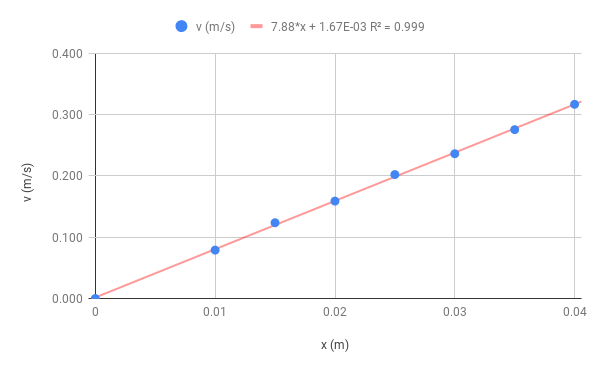
\includegraphics[scale=0.71]{image/06-kinetic/v.png}
    \caption{Velocity versus distance from equilibrium}
    \label{figure:06.v}
\end{figure}
%%%%%%%%%%%%%%%%%%%%%%%%%%%%%%%%%%%%%%%%%%%%%%%%%%%%%%%%%%%%%%%%%%%%%%%%%%%%%%%%
\begin{figure}[ht]
    \centering
    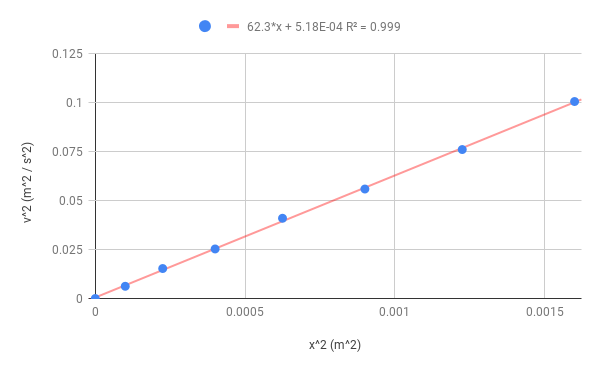
\includegraphics[scale=0.71]{image/06-kinetic/v2.png}
    \caption{Square of Velocity versus square of distance from equilibrium}
    \label{figure:06.v.2}
\end{figure}
%%%%%%%%%%%%%%%%%%%%%%%%%%%%%%%%%%%%%%%%%%%%%%%%%%%%%%%%%%%%%%%%%%%%%%%%%%%%%%%%